\documentclass[12pt]{article}
\usepackage[utf8]{inputenc}
\usepackage[a4paper,left=3cm,right=2cm,top=2.5cm,bottom=2.5cm]{geometry}
\usepackage{amsmath}
\usepackage{listings}

\title{Signal and Image Processing: Homework 04}
\author{Patomporn Payoungkhamdee 6138171}
\date{\today}

\usepackage{placeins}
\usepackage{natbib}
\usepackage{graphicx}

\begin{document}

\maketitle

1. Consider a discrete-time system described by the difference equation

\begin{equation*}
y(k) = y(k-1) - 0.24y(k-2) + 2x(k-1) - 1.6x(k-2)
\end{equation*}

1.1) Find the transfer function ($H(z)$)
\begin{equation*}
\begin{split}
    H(z) &= \frac{2z^{-1} - 1.6z^{-2}}{1-z^{-1}+0.2z^{-2}} \\
    &= \frac{2(z-0.8)}{(z-0.6)(z-0.4)}
\end{split}
\end{equation*}

1.2) Write down the form of the natural mode terms of this system

\begin{equation*}
y_\text{natural}(k) = c_1(0.6)^k\mu(k) + c_2 (0.4)^k\mu(k)
\end{equation*}

1.3) Find zero-state response to input $x(k) = 10\mu(k)$

Since there are two simple poles, then
\begin{equation*}
    c_1 = \left.\frac{10(z-p_i)2(z-0.8)}{(z-1)(z-0.6)(z-0.4)}\right|_{z=p_i}
\end{equation*}

\begin{equation*}
\begin{split}
c_0 &= \frac{20(0.2)}{0.4(0.6)} = \frac{50}{3} \\
c_1 &= \frac{20(-0.2)}{(-0.4)(0.2)} = 50 \\
c_2 &= \frac{20(-0.4)}{(-0.6)(-0.2)} = -\frac{200}{3} 
\end{split}
\end{equation*}
Hence
\begin{equation*}
    y_\text{zs}(k) = \frac{50}{3}\mu(k) + 50(0.6)^k\mu(k) - \frac{200}{3}(0.4)^k\mu(k)
\end{equation*}

1.4) Causal exponential input $x(k) = (0.8)^k\mu(k)$. Applying Z-TF as
\begin{equation*}
    X(z) = \frac{z}{z-0.8}
\end{equation*}
From
\begin{equation*}
    Y(z) = H(z)X(z) = \frac{2z}{(z-0.6)(z-0.4)}
\end{equation*}
Finding 
\begin{equation*}
    y_\text{zs}(k) = Z^{-1}\{Y(z)\}
\end{equation*}

From Initial value theorem,\
\begin{equation*}
    y(0) = \lim_{z\rightarrow\infty}Y(z) = 0
\end{equation*}
Finding residue on each simple poles by using
\begin{equation*}
    \text{Res}(p_i, k) = \left.(z-p_i)Y(z)z^{k-1}\right|_{z=p_i}
\end{equation*}
Calculating the residue in our case
\begin{equation*}
\begin{split}
    \text{Res}(0.6, k) &= \frac{2(0.6)^k}{0.2} = 10 (0.6)^k \\
    \text{Res}(0.6, k) &= \frac{2(0.6)^k}{-0.2} = -10 (0.4)^k
\end{split}
\end{equation*}

\begin{equation*}
    y_\text{zs}(k) = [10(0.6)^k - 10(0.4)^k]\mu(k-1)
\end{equation*}

Force modes are basically generated by poles of $X(z)$.
Let interpret $Y(z)=H(z)X(z)$ where pole $z=q$ of $X(z)$ match 
zero $z=q$ of $H(z)$ calling "pole-zero cancellation" where it 
prevent force mode that could appear in $y(k)$.

1.5) Causal input $x(k)=(0.4)^k\mu(k)$, then
\begin{equation*}
\begin{split}
    X(z) &= Z\{x(k)\} \\
        &= \frac{z}{z-0.4}
\end{split}
\end{equation*}
The output in z-domain be represented as
\begin{equation*}
\begin{split}
    Y(z) &= H(z)X(z) = \frac{2z(z-0.8)}{(z-0.6)(z-0.4)^2} \\
    \text{and}\ y(k) &= Z^{-1}\{Y(z)\}
\end{split}
\end{equation*}

Zero-state response of is in the form of
\begin{equation*}
    y_\text{zs}(k) = y_0\delta(k) + [\sum_{i=1}^n \text{Res}(p_i, k)]\mu(k-1)    
\end{equation*}
From initial value theorem,
\begin{equation*}
    y(0) = \lim_{z\rightarrow\infty}Y(z) = 0
\end{equation*}
Calculating the residue of each poles
\begin{equation*}
\begin{split}
    \text{Res}(0.6, k) &= \left.\frac{(z-0.6)2(z-0.8)z^k}{(z-0.6)(z-0.4)^2}\right|_{z=0.6} \\
    &= -10(0.6)^k
\end{split}
\end{equation*}
\begin{equation*}
\begin{split}
    \text{Res}(0.4, k) &= \left.\frac{d}{dz}\frac{(z-0.4)^2 2(z-0.8)z^k}{(z-0.6)(z-0.4)^2}\right|_{z=0.6} \\
    &= 0
\end{split}
\end{equation*}
Hence
\begin{equation*}
\begin{split}
    y_\text{zs} (k) &= -10(0.6)^k\mu(k-1)
\end{split}
\end{equation*}
This is an example of harmonic forcing where pole of $X(z)$ is located
at the same point of pole of $H(z)$ on the complex plane.

\vspace{20pt}
2. Consider a discrete-time system described by the following transfer function
\begin{equation*}
    H(z) = \frac{3(z-0.4)}{z+0.8}
\end{equation*}

2.1) Support $y_\text{zs}(k) = \mu(k)$ to $x(k)$ find $X(z)$.
\begin{equation*}
    \begin{split}
        Y(z) &= Z\{y_\text{zs}(k)\} = Z\{\mu(k)\} \\
        &= \frac{z}{z-1}
    \end{split}
\end{equation*}
From 
\begin{equation*}
    \begin{split}
        Y(z) &= H(z)X(z) \\
        X(z) &= H(z)/Y(z) \\
        &= \frac{3(z-0.4)(z-1)}{z(z+0.8)}
    \end{split}
\end{equation*}

2.2) Find $x(k)=Z^{-1}\{X(z)\}$

Initial value theorem, $x(0)=\lim_{z\rightarrow\infty}X(z)=3$.
Finding the residue from two simple poles by using form
\begin{equation*}
\begin{split}
    \text{Res}(p_i, k) &= (z-p_i)X(z)z^{k-1}|_{z=p_i} \\
    &= \left.\frac{3(z-p_i)(z-0.4)(z-1)z^{k-1}}{z(z+0.8)}\right|_{z=p_i} \\
\end{split}
\end{equation*}
then
\begin{equation*}
    \text{Res}(0, k) = \left.\frac{3(-0.4)(-1)}{0.8}z^{k-2}\right|_{z=0} = \frac{3}{2}\delta(k-2)
\end{equation*}

\begin{equation*}
    \text{Res}(-0.8, k) = \frac{3(-1.2)(-1.8)}{-0.8}(0.8)^{k-2} = 6.48(0.8)^{k-1}
\end{equation*}
Then zero-state response is
\begin{equation*}
    y_\text{zs}(k) = 3\delta(k) + \frac{3}{2}\delta(k-2) + 6.48(0.8)^{k-1}\mu(k-1)
\end{equation*}


\vspace{20pt}
3. Consider the following discrete-time signal $x = [1,2,1,0]^T$

3.1) Find $X(i) = \text{DFT}\{x(k)\}$

In this case $N=4$, 
\begin{equation*}
    X(i) = \sum_{k=0}^3 x(k)\exp(-j2\pi ik/N)
\end{equation*}
\begin{equation*}
\begin{split}
    X(i) &= 1 + 2\exp(-j\pi i/2) + \exp(-j\pi i) \\
    &= [1+2\cos(\pi i/4) + \cos(\pi i)] - i [2\sin(\pi i/4) + \sin(\pi i)]
\end{split}
\end{equation*}

3.2) Magnitude of the spectrum $A_x(i) = 2|X(i)|/N$.

Let's begin with finding $|X(i)|$ as
\begin{equation*}
\begin{split}
    |X(i)| &= \sqrt{[1+2\cos(\pi i/2)+\cos(\pi i)]^2 + [2\sin(\pi i/2) + \sin(\pi i)]^2} \\
    &= \sqrt{6 + 4\cos(\pi i) + 2\cos(\pi i/2) + 4\cos(\pi i/2)} \\
    &= \sqrt{6[1+\cos(\pi i/2)] + 4\cos(\pi i)}
\end{split}
\end{equation*}
So,
\begin{equation*}
    A_x(i) = \frac{1}{2}\sqrt{6[1+\cos(\pi i/2)] + 4\cos(\pi i)}
\end{equation*}

3.3) Phase spectrum $\phi_x(i)$
\begin{equation*}
    \phi(x) = \arctan\left(\frac{2\sin(\pi i/2)+\sin(\pi i)}{1+2\cos(\pi i/2)+\cos(\pi i)}\right)
\end{equation*}

3.4) Power density spectrum $S_x(i) = |X(i)|^2/N$
\begin{equation*}
    S_x(i) = \frac{1}{3}\left\{6[1+\cos(\pi i/2)] + + 4\cos(\pi i)\right\}
\end{equation*}

3.5) Verify Parseval's indentity $\sum_{k=0}^3|x(k)| = (1/4)\sum_{i=0}^3|X(i)|^2$

Let compute LHS
\begin{equation*}
    \sum_{k=0}^3|x(k)| = 1 + 4 + 1 = 6
\end{equation*}
and the RHS
\begin{equation*}
\begin{split}
    (1/4)\sum_{i=0}^3|X(i)|^2 &= \frac{1}{4}\{ [6 (1+1) + 4] \\
    &\ + [6(1-0)-4] \\
    &\ + [6(1-1)+4] \\
    &\ + [6(1-0)-4]\} \\
    &= 24/4 = 6
\end{split}
\end{equation*}

\vspace{20pt}
4. Let $x_a(t)$ to be a periodic pulse train of period $T_0= 1$.
Suppose the pulse amplitude is $a=10$ and the pulse duration is
$\tau=T/5$ This signal can be represented by
the Fourier series

The result has shown in figure [1-3]

\begin{figure}[h!]
    \centering
    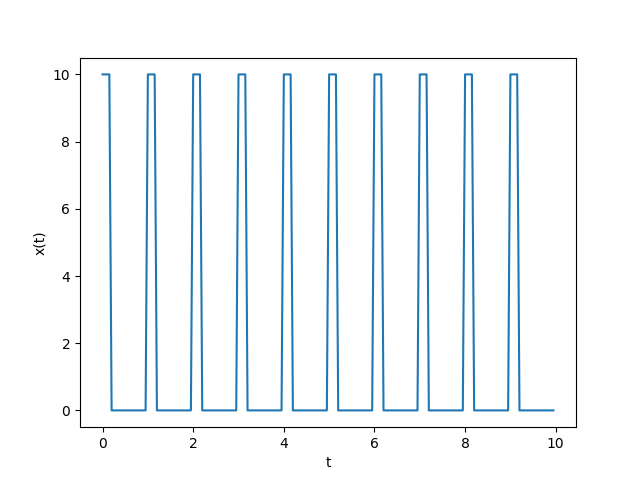
\includegraphics[width=0.8\linewidth]{../pb4_x}
    \caption{Figure of signal}
\end{figure}
\begin{figure}[h!]
    \centering
    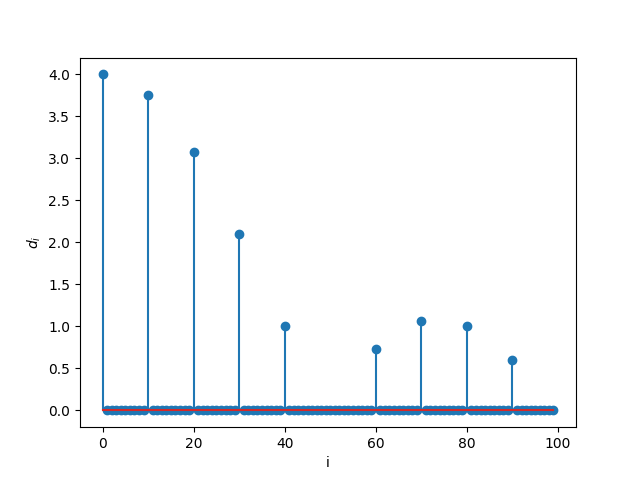
\includegraphics[width=0.8\linewidth]{../pb4_d}
    \caption{Figure of fourier coefficient}
\end{figure}
\begin{figure}[h!]
    \centering
    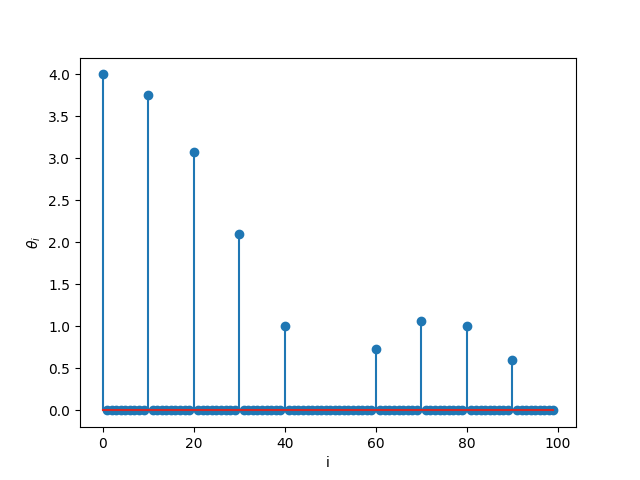
\includegraphics[width=0.8\linewidth]{../pb4_p}
    \caption{Figure of the phase}
\end{figure}

\FloatBarrier
\begin{lstlisting}
    import typing
    import math
    import numpy as np
    
    
    import matplotlib
    matplotlib.use('TkAgg')
    import matplotlib.pyplot as plt
    
    
    T0 = 1
    A = 10.0
    T = T0/float(5)
    N = 128
    M = 16
    
    FS = 20
    SAMPLING_FREQ = 1.0/float(FS)
    
    def x(k: int) -> float:
        t = float(k) * SAMPLING_FREQ
        if t % T0 < T:
            return A
        return 0.0
    
    def X(i: int, _wn: complex) -> float:
        wn_vec = np.vectorize(lambda k: _wn**(i*k))(range(N))
        x_vec = np.vectorize(lambda k: x(k))(range(N))
        return np.dot(x_vec, wn_vec)
    
    def d(i: int, _wn: complex) -> float:
        return 2.0*np.abs(X(i, _wn))/float(N)
    
    def phase(i: int, _wn: complex) -> float:
        return np.angle(X(i, _wn))
    
    if __name__ == "__main__":
        i = [float(i) * SAMPLING_FREQ for i in range(N)]
        x_vec = np.vectorize(lambda k: x(k))(range(N))
        plt.plot(i, x_vec)
        plt.xlabel("t")
        plt.ylabel("x(t)")
        plt.savefig("pb4_x.png")
        plt.cla()
        plt.clf()
        # plt.show()
    
        wn = np.exp(complex(0, -2.0*math.pi/float(N)))
        X_vec = np.vectorize(lambda i: X(i, wn))(range(N))
    
        d_vec = [d(i, wn) for i in range(M)]
        plt.stem(d_vec)
        plt.xlabel("i")
        plt.ylabel(r"$d_i$")
        plt.savefig("pb4_d.png")
        plt.cla()
        plt.clf()
    
        phase_vec = [phase(i, wn) for i in range(M)]
        plt.stem(d_vec)
        plt.xlabel("i")
        plt.ylabel(r"$\theta_i$")
        plt.savefig("pb4_p.png")
        plt.cla()
        plt.clf()
\end{lstlisting}

\FloatBarrier
\vspace{20pt}
5. Consider the following noisy periodic signal with a sampling
frequency of $f_s= 1600$ Hz and $N= 1024$
\begin{equation*}
    x(k) = \sin^2(400\pi kT)\cos^2(300pi kT) + \mathcal{N}(0, 1/\sqrt{2})
\end{equation*}


5.1) Compute and plot the power density spectrum as in figure 4
\begin{figure}[h!]
    \centering
    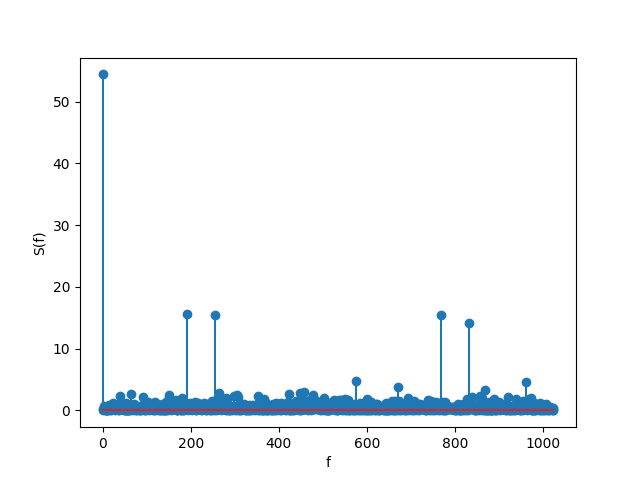
\includegraphics[width=\linewidth]{../pb5_1}
    \caption{Figure of spectrum frequency}
\end{figure}

5.2) Compute and print the average power

and the result looks like
\begin{lstlisting}
    Average power of x(i):  0.626707818480065
    Average power of moise:  0.5034344200386078
\end{lstlisting}

\FloatBarrier
Source code
\begin{lstlisting}
    import typing
    import math
    import numpy as np
    
    
    import matplotlib
    matplotlib.use('TkAgg')
    import matplotlib.pyplot as plt
    
    
    FS = 1600
    N = 1024
    T = 1.0/float(FS)
    
    INV_SQRT2 = 1.0/math.sqrt(2)
    
    def x(k: int) -> float:
        _k = float(k)
        _x = (np.sin(400.0*math.pi*_k*T)**2 \
            * np.cos(300.0*math.pi*_k*T)**2) \
            + np.random.normal(0.0, INV_SQRT2)
        return _x
    
    def X(i: int, _wn: complex) -> float:
        wn_vec = np.vectorize(lambda k: _wn**(i*k))(range(N))
        x_vec = np.vectorize(lambda k: x(k))(range(N))
        return np.dot(x_vec, wn_vec)
    
    def pb51():
        wn = np.exp(complex(0, -2.0*math.pi/float(N)))
        Wn_vec = np.vectorize(lambda i: X(i, wn))(range(N))
        Sx_vec = np.abs(Wn_vec)**2.0 / float(N)
        plt.stem(range(N), Sx_vec)
        plt.ylabel("S(f)")
        plt.xlabel("f")
        plt.savefig("pb5_1.png")
        # plt.show()
    
    def pb52():
        x_vec = np.vectorize(lambda k: x(k))(range(N))
        avg_pow_x = np.mean(np.square(x_vec))
        print("Average power of x(i): ", avg_pow_x)
        noise = np.random.normal(0.0, INV_SQRT2, size=N)
        avg_pow_noise = np.mean(np.square(noise))
        print("Average power of moise: ", avg_pow_noise)
    
    if __name__ == "__main__":
        pb51()
        pb52()

\end{lstlisting}


\end{document}
